\section{Fonctions du message}

\begin{frame}
	\frametitle{Les types de messages}
	\begin{block}{Skinner (1947)}
		\begin{itemize}
			\item{Les demandes}
			\item{Les dénominations}
		\end{itemize}
	\end{block} \pause
	
	\begin{exampleblock}{Exemple}
		\begin{itemize}
			\item{"Ma poupée"}
			\item{"Donne-moi ma poupée" : demande}
			\item{"Voici ma poupée" : dénomination}
		\end{itemize}
	\end{exampleblock}
\end{frame}


\begin{frame}
	\frametitle{Les types de communication}
	\begin{block}{Zajonc (1966)}
		\begin{itemize}
			\item{Communication incidente} \pause
			\item{Communication consommatoire} \pause
			\item{Communication instrumentale}
		\end{itemize}
	\end{block}
\end{frame}


\begin{frame}
	\frametitle{Les fonctions du message}
	\begin{block}{Jakobson (1958)}
		\begin{center}
		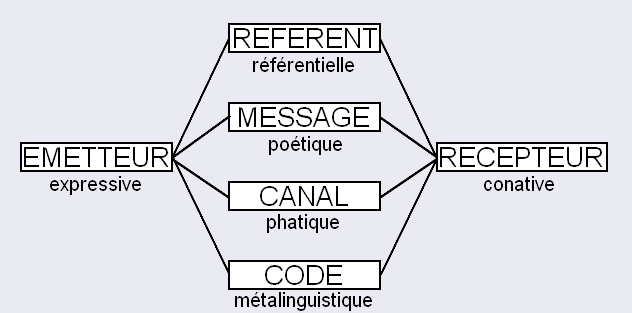
\includegraphics[height=4cm]{jakobson.png}
		\end{center}
	\end{block} \pause
	
	\begin{block}{Jakobson (1958)}
		\begin{columns}
			\begin{column}{.5\textwidth}
				\begin{itemize}
					\item{Fonction expressive} \pause
					\item{Fonction conative} \pause
					\item{Fonction référentielle} \pause
				\end{itemize}
			\end{column}
			\begin{column}{.5\textwidth}
				\begin{itemize}
					\item{Fonction phatique} \pause
					\item{Fonction métalinguistique} \pause
					\item{Fonction poétique}
				\end{itemize}
			\end{column}
		\end{columns}
	\end{block}
\end{frame}
